\documentclass[sigconf,nonacm]{acmart}
\settopmatter{printacmref=false,printfolios=true}
\renewcommand\footnotetextcopyrightpermission[1]{}
\pagestyle{plain}

\usepackage{booktabs}
\usepackage{array}
\usepackage{tikz}
\usetikzlibrary{arrows.meta,positioning,fit,calc}
\usepackage{pgfplots}
\pgfplotsset{compat=1.17}

\newcommand{\us}{\,$\mu$s}

\begin{document}

\title{Does Kernel-Owned Networking Make GPU Serving Cheaper?}
\subtitle{Lessons from an eBPF-Driven GPU Server}

\author{Yusheng Zheng}
\affiliation{%
  \institution{UC Santa Cruz}
  \city{Santa Cruz}
  \state{CA}
  \country{USA}}
\email{yzhen165@ucsc.edu}

\begin{abstract}
A tempting design for small-model GPU serving removes the userspace request
loop entirely: eBPF frames and admits requests arriving on ordinary Linux TCP
sockets, a resident GPU dispatcher executes CUDA graphs, and a BPF program
driving io\_uring sends the replies. We built such a system, bpf-gpu-server, on stock
Linux~7.3 without a kernel module, and compared it with an efficient C++ epoll
server that drives the same GPU executor. Across LLM serving with
Qwen2.5-0.5B and high-rate cuBLAS/cuFFT requests (more than 3.4 million
measured requests in the final experiments), moving the request loop into the
kernel did not reduce latency or total CPU. Throughput was identical, and
per-request CPU moved from user to system time (11.3+26.2\us{} versus
2.8+35.2\us). The large improvements we found, a 15$\times$ lower completion
tail from adding GPU slots and a 17$\times$ lower token-gap tail from disabling
Nagle's algorithm, apply equally to both transports. The kernel TCP stack and
completion coordination dominate per-request cost, and both remain on the
kernel-owned path.
\end{abstract}

\maketitle

\section{Introduction}

Serving a small model, or a short GPU kernel, at a high request rate makes host
overhead visible. Each request still crosses the network stack, wakes a server
thread, is copied into user memory, is queued for the GPU, and returns through
another send. When the computation itself takes microseconds to a few
milliseconds, this shepherding can be a large share of the work.

Two recent Linux capabilities suggest removing the shepherd. Sockmap BPF
programs can parse and steer data on TCP sockets inside the kernel, and Linux
7.3 lets a sleepable BPF program submit and complete io\_uring operations
itself. Combined with a persistent GPU dispatcher that launches captured CUDA
graphs without host involvement, a server needs userspace only at startup:
after initialization no user thread reads, schedules or sends a request.
Intuitively this should save CPU and shorten tails, because it skips system
calls, user copies and thread wakeups.

We built this design as bpf-gpu-server and asked a narrow question: \emph{compared
with a well-engineered userspace server that drives the same GPU executor, does
kernel-owned networking reduce CPU or latency?} The answer on our testbed is
no. This paper reports:

\begin{itemize}
\item a working kernel-owned TCP-to-GPU serving path on stock Linux, validated
with real models and unchanged cuBLAS/cuFFT graphs (\S\ref{sec:design});
\item a controlled comparison that changes only the transport, plus an
external vLLM reference and explicit CPU accounting (\S\ref{sec:method});
\item a negative result for throughput, tail latency and total CPU, together
with an explanation of where the cost goes (\S\ref{sec:results},
\S\ref{sec:why});
\item transport-independent fixes that mattered far more than the transport
(\S\ref{sec:fixes}).
\end{itemize}

\section{Design}
\label{sec:design}

\begin{figure}[t]
\centering
\resizebox{\columnwidth}{!}{%
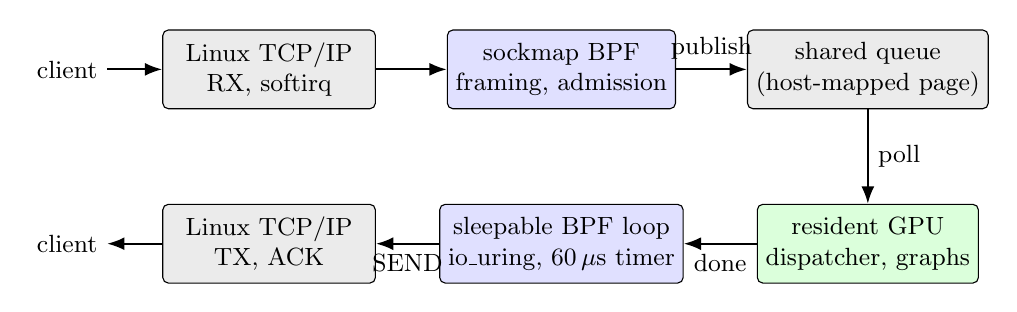
\begin{tikzpicture}[
  font=\small,
  box/.style={draw,rounded corners=2pt,align=center,minimum height=10mm,minimum width=27mm,inner sep=3pt},
  bpf/.style={box,fill=blue!12},
  nat/.style={box,fill=black!8},
  gpu/.style={box,fill=green!14},
  arr/.style={-{Latex[length=2.2mm]},thick}]
\node[nat] (tcpin) {Linux TCP/IP\\RX, softirq};
\node[bpf,right=9mm of tcpin] (sk) {sockmap BPF\\framing, admission};
\node[nat,right=9mm of sk] (q) {shared queue\\(host-mapped page)};
\node[gpu,below=12mm of q] (g) {resident GPU\\dispatcher, graphs};
\node[bpf,below=12mm of sk] (loop) {sleepable BPF loop\\io\_uring, 60\us{} timer};
\node[nat,below=12mm of tcpin] (tcpout) {Linux TCP/IP\\TX, ACK};
\node[left=7mm of tcpin] (cin) {client};
\node[left=7mm of tcpout] (cout) {client};
\draw[arr] (cin) -- (tcpin);
\draw[arr] (tcpin) -- (sk);
\draw[arr] (sk) -- node[above]{publish} (q);
\draw[arr] (q) -- node[right]{poll} (g);
\draw[arr] (g) -- node[below]{done} (loop);
\draw[arr] (loop) -- node[below]{SEND} (tcpout);
\draw[arr] (tcpout) -- (cout);
\end{tikzpicture}}
\caption{Steady-state path of the kernel-owned transport. Blue boxes are eBPF,
gray boxes are native kernel code, green is GPU. Userspace appears only at
startup. The comparator replaces both blue boxes with one C++ epoll thread
and keeps everything else.}
\label{fig:arch}
\end{figure}

At startup a userspace process creates the listening socket, captures the
caller's CUDA graphs, maps a shared page that both the CPU and GPU can access,
attaches the BPF programs, and launches a resident GPU dispatcher. It then stays
alive only to own these allocations and to handle shutdown.

Figure~\ref{fig:arch} shows the steady state. Linux TCP reassembles bytes as
usual. A sockmap BPF program frames each request (a 24-byte header followed by
32-bit words, optionally wrapped in a Content-Length HTTP POST), validates it,
and publishes it into a FIFO in the shared page. The GPU dispatcher reads
published requests with system-scope acquire loads, launches the matching
caller-owned graph, and publishes outputs. Two compute adapters exist: an opaque
one-shot adapter for unchanged cuBLAS and cuFFT graphs, and a generation adapter
that replays upstream vLLM or Hugging Face prefill and decode graphs for
Qwen2.5-0.5B and SmolLM2-135M. A sleepable BPF program attached to io\_uring
consumes completions, submits SEND operations for finished outputs, preserves
reply ordering, and reclaims connections. While work is active it waits for the
next completion event or a 60\us{} timer.

Some parts of the path remain native kernel code, and they matter for the
results: TCP/IP processing with its interrupts and softirqs, the io\_uring core
and its io-wq workers, and the thread context in which the BPF loop runs, which
belongs to the service process.

\section{Methodology}
\label{sec:method}

\paragraph{Baselines.} The main comparator, \emph{native}, uses the same queue,
the same GPU dispatcher and the same graphs, but replaces the two BPF components
with a C++ thread that uses timed epoll and nonblocking reads and writes. Only
the transport placement differs. Official vLLM~0.31~\cite{vllm} with its optimized defaults
serves as an external reference for the LLM workload; its HTTP API, scheduler
and KV management differ, so it measures the whole serving design rather than
the transport.

\paragraph{Testbed.} The server has an Intel Core Ultra~9 285K (24 logical
CPUs), an RTX~5090 and Linux 7.3-rc3. Load comes from a client on a separate
host. Every condition runs in five paired process blocks with counterbalanced
order; we report means of block statistics with nominal paired 95\% intervals.

\paragraph{Workloads.} \emph{LLM}: Qwen2.5-0.5B in FP16, short prompts, 64
output tokens, 192 requests/s for 60\,s (12,288 offered tokens/s).
\emph{Small graphs}: an 8$\times$8 FP32 cuBLAS GEMM or a 32-point complex64
cuFFT, repeated 1, 16 or 256 times inside a graph, with 280-byte requests,
256-byte replies and 128 persistent connections. A 60-cell screen over work
size, offered rate up to saturation and service CPU affinity (1, 2 or all
logical CPUs) covered 2.52 million requests. Three points selected by a fixed
rule were then confirmed with new seeds (600,000 requests). The success
criterion was fixed in advance: an upper 95\% bound on the CPU ratio below 0.90
with a P99 bound no worse than 1.05, or the reverse, and throughput no worse
than 0.98.

\paragraph{CPU accounting.} \emph{Process-group CPU} is user plus system time
charged to the service's threads, including io-wq. Softirq work charged to
other contexts and whole-host totals are reported separately and never summed
with it. Outputs are checked by exact replay; failures and timeouts are kept in
all statistics.

\section{Results}
\label{sec:results}

\subsection{LLM serving: the transport does not matter}

\begin{table}[t]
\centering
\small
\caption{Qwen2.5-0.5B at 192 requests/s. Top: transport comparison with 16 GPU
slots. Bottom: a separate run that raises common capacity to 32 slots
(native transport). CPU is process-group CPU per request.}
\label{tab:llm}
\begin{tabular}{lrrr}
\toprule
Path & tokens/s & P99 (ms) & CPU (ms) \\
\midrule
Kernel-owned, 16 slots & 11,645 & 3,304 & 0.835 \\
Native epoll, 16 slots & 11,645 & 3,314 & 0.812 \\
Official vLLM & 12,245 & 611 & 8.545 \\
\midrule
Native epoll, 16 slots & 11,640 & 3,337 & 0.751 \\
Native epoll, 32 slots & 12,265 & 217 & 0.523 \\
Official vLLM & 12,249 & 406 & 8.327 \\
\bottomrule
\end{tabular}
\end{table}

The top half of Table~\ref{tab:llm} compares the two transports over 172,800
requests with no failures. Throughput is identical, and the differences in
completion P99 ($-10$\,ms, interval $[-64, 44]$) and process CPU cross zero.
An earlier variant of the kernel path measured 18.7\% lower process-group CPU than native after the polling fix in
\S\ref{sec:fixes}. That difference did not reproduce in the final integrated
path and never appeared in whole-host CPU.

Both resident paths had a multi-second tail while vLLM stayed near 0.6\,s. The
cause was capacity, not transport. With 16 slots the offered load exceeded
delivery, so the queue grew for the whole run: native time to first token rose
from about 235\,ms in the first 10\,s to 3,003\,ms in the last 10\,s, while
generation stayed near 86\,ms. Raising common capacity to 32 slots (bottom
half) cut P99 from 3,337 to 217\,ms, below vLLM's 406\,ms at equal throughput.
It also cost 0.033\,ms of mean time per token, more graph and KV memory, and
0.34\,J more device energy per request than vLLM.

The resident executor also used 10--16$\times$ less process CPU per request
than the vLLM server. Most of that gap comes from moving step scheduling onto
the GPU and from a simpler protocol that returns token IDs instead of JSON
text, and both transports share it. Kernel networking does not explain it.

\subsection{Small requests: no CPU or tail benefit}

\begin{table}[t]
\centering
\small
\caption{Confirmation at 1,000 requests/s (five pairs each). Ratios are
kernel-owned over native; values below 1 favor the kernel path.}
\label{tab:small}
\begin{tabular}{lcc}
\toprule
Point & CPU ratio [95\%] & P99 ratio [95\%] \\
\midrule
FFT, all CPUs & 1.011 [0.995, 1.027] & 1.254 [0.514, 3.058] \\
GEMM, all CPUs & 1.019 [0.967, 1.074] & 1.160 [0.497, 2.706] \\
GEMM, one CPU & 1.129 [0.956, 1.334] & 2.589 [1.196, 5.607] \\
\bottomrule
\end{tabular}
\end{table}

Short GPU work is where host overhead should matter most, yet no point met the
success criterion (Table~\ref{tab:small}). The largest CPU reduction anywhere in
the screen was about 5.8\%, and with one logical CPU the kernel path's P99 was
2.6$\times$ worse. Whole-host CPU ratios (0.990, 0.925 and 0.988) all had
intervals crossing 1. Both transports first saturated at the same offered
level. Longer GPU work narrowed throughput gaps without producing a CPU
advantage. All 3.12 million requests completed without an observed failure.

\begin{figure}[t]
\centering
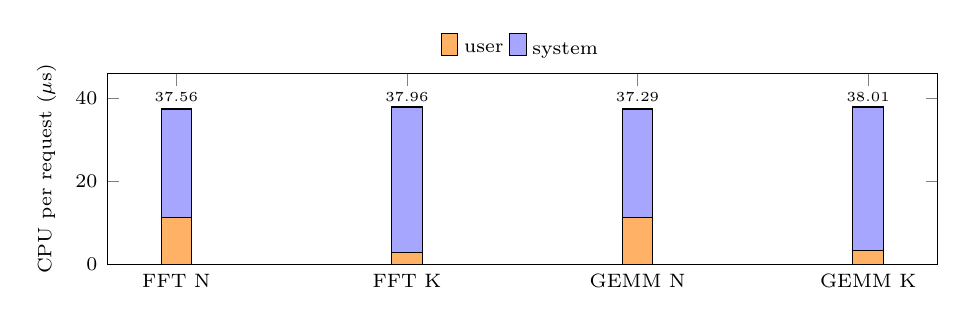
\begin{tikzpicture}
\begin{axis}[
  ybar stacked, bar width=11pt, height=4.0cm, width=\columnwidth,
  ymin=0, ymax=46, ylabel={CPU per request ($\mu$s)},
  symbolic x coords={FFT N,FFT K,GEMM N,GEMM K},
  xtick=data, tick label style={font=\scriptsize}, label style={font=\scriptsize},
  legend style={font=\scriptsize,at={(0.5,1.02)},anchor=south,legend columns=2,draw=none},
  nodes near coords style={font=\tiny}]
\addplot[fill=orange!60] coordinates {(FFT N,11.3) (FFT K,2.8) (GEMM N,11.3) (GEMM K,3.3)};
\addplot[fill=blue!35] coordinates {(FFT N,26.2) (FFT K,35.2) (GEMM N,26.2) (GEMM K,34.7)};
\legend{user, system}
\node[font=\tiny] at (axis cs:FFT N,40.5) {37.56};
\node[font=\tiny] at (axis cs:FFT K,40.5) {37.96};
\node[font=\tiny] at (axis cs:GEMM N,40.5) {37.29};
\node[font=\tiny] at (axis cs:GEMM K,40.5) {38.01};
\end{axis}
\end{tikzpicture}
\caption{Process-group CPU per request at 1,000 requests/s, native (N) versus
kernel-owned (K). Bars are coarse tick-based user/system splits; numbers on
top are high-resolution totals. Removing the userspace loop moves work into
system time.}
\label{fig:cpu}
\end{figure}

Figure~\ref{fig:cpu} shows why. The kernel path cut user time from 11.3 to
2.8\us{} per request, but system time grew from 26.2 to 35.2\us. The totals
stayed within about 1\%.

\subsection{Fixes that mattered more than the transport}
\label{sec:fixes}

\begin{table}[t]
\centering
\small
\caption{Before/after effects of individual fixes (LLM workload). ``Both''
means the fix and its gain apply to both transports.}
\label{tab:fixes}
\begin{tabular}{@{}>{\raggedright\arraybackslash}p{0.27\columnwidth}l>{\raggedright\arraybackslash}p{0.50\columnwidth}@{}}
\toprule
Fix & Scope & Effect \\
\midrule
TCP\_NODELAY & both & token-gap P99 40.5$\to$2.3\,ms; tokens/s 8,842$\to$11,260 \\
EOF reclamation & kernel & failed requests 4,157$\to$0 of 57,600; tokens/s 7,793$\to$11,623 \\
Active-wait polling & kernel & process CPU 1.70$\to$0.63\,ms per request \\
Mixed prefill and decode~\cite{sarathi} & both & mean time per token 1.43$\to$1.23\,ms ($-14\%$) \\
16$\to$32 GPU slots & both & completion P99 3,337$\to$217\,ms \\
\bottomrule
\end{tabular}
\end{table}

Table~\ref{tab:fixes} lists the changes with the largest measured effects. Two
are general lessons for anyone writing a TCP front end for a GPU. First,
streamed small replies interact badly with Nagle's algorithm and delayed ACKs:
a 4-byte write left 36 queued bytes waiting about 41\,ms for an ACK, so every
stream paid a 40\,ms gap until the listener set TCP\_NODELAY. Second, under
sustained load the kernel path kept finished connections until an unrelated
global queue drained; 2,947 sockets sat in CLOSE\_WAIT, the sockhash filled, and
new requests failed with E2BIG. Per-connection reclamation removed all 4,157
timeouts. A third fix removed a busy-polling branch in the BPF loop, where 71\%
of the loop thread's kernel samples had been coordination and BPF map
operations.

\section{Why the Kernel Path Saves No CPU}
\label{sec:why}

\paragraph{The expensive part stays.} Per request, the dominant cost is TCP/IP
processing: interrupts and softirqs on receive, socket buffers, the state
machine, ACKs and transmission. Sockmap runs after TCP has reassembled the
stream, so both transports pay for the full stack. What the kernel path removes
is the system call boundary and one user copy, which is a small fraction of the
roughly 38\us{} each request costs on this host.

\paragraph{The worker moves rather than disappears.} Someone must notice that
the GPU has finished and submit the reply. The GPU cannot cheaply trigger
kernel work, so the BPF loop runs in a service thread that waits for completion
events or a 60\us{} timer, reads queue state through BPF maps, and submits
SQEs. Its time is charged as system time, which is exactly the shift in
Figure~\ref{fig:cpu}. An epoll server batches many ready sockets per system
call, while the BPF path pays for program invocations, map operations and
SQE/CQE handling on every request.

Figure~\ref{fig:profile} makes this concrete for the LLM workload before the
active-wait fix. The native thread spends 85\% of its kernel samples in
networking and softirq, which is the work both designs must do. The
kernel-owned thread was on CPU four times as often, and 71\% of its kernel
samples were loop coordination and BPF map operations that the native design
does not have. The fix in \S\ref{sec:fixes} removed most of this extra work
for LLM serving, but in the small-request experiment the remaining
coordination still cancelled the user-time savings.

\begin{figure}[t]
\centering
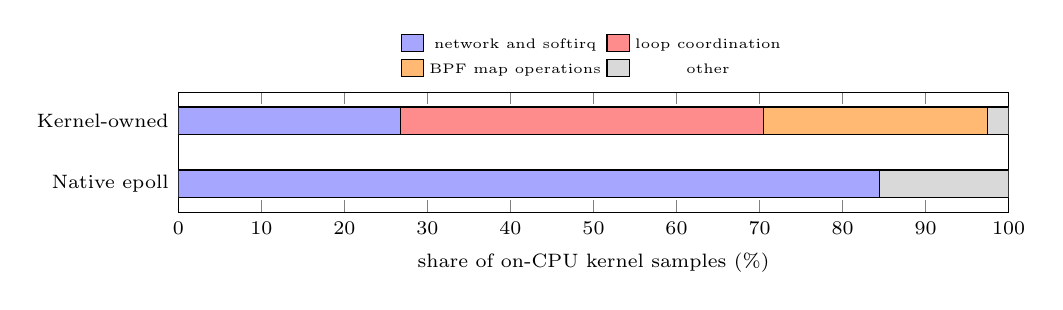
\begin{tikzpicture}
\begin{axis}[
  xbar stacked, bar width=10pt, height=3.1cm, width=\columnwidth,
  xmin=0, xmax=100, xlabel={share of on-CPU kernel samples (\%)},
  symbolic y coords={Native epoll,Kernel-owned}, ytick=data,
  tick label style={font=\scriptsize}, label style={font=\scriptsize},
  legend style={font=\tiny,at={(0.5,1.03)},anchor=south,legend columns=2,draw=none},
  enlarge y limits=0.45]
\addplot[fill=blue!35] coordinates {(26.7,Kernel-owned) (84.5,Native epoll)};
\addplot[fill=red!45] coordinates {(43.8,Kernel-owned) (0,Native epoll)};
\addplot[fill=orange!55] coordinates {(27.0,Kernel-owned) (0,Native epoll)};
\addplot[fill=black!15] coordinates {(2.5,Kernel-owned) (15.5,Native epoll)};
\legend{network and softirq, loop coordination, BPF map operations, other}
\end{axis}
\end{tikzpicture}
\caption{Where the service thread's kernel samples go (perf at 499\,Hz, LLM
workload at 192 requests/s, before the active-wait fix). The kernel-owned
thread also had 4.1$\times$ more on-CPU samples (10,086 versus 2,455).}
\label{fig:profile}
\end{figure}

\paragraph{Fewer cores make it worse.} With one logical CPU the loop competes
with network softirqs, and timer-driven wakeups add delay that readiness-driven
epoll avoids, which matches the 2.6$\times$ worse P99.

\paragraph{When moving into the kernel does pay off.} eBPF systems with large
gains intercept work \emph{before} the expensive layers: BMC~\cite{bmc} and
Electrode~\cite{electrode} act at XDP~\cite{xdp} before the network stack, and
XRP~\cite{xrp} resubmits storage requests from the NVMe driver. GPU networking
systems that remove the CPU from the data path bypass the host stack entirely,
through RDMA in GPUnet~\cite{gpunet} or direct NIC queues in DOCA
GPUNetIO~\cite{gpunetio}. Keeping ordinary Linux TCP, as bpf-gpu-server does for
compatibility, means accepting the stack's cost on every request.

\section{Related Work}

\emph{GPU-side I/O and services.} GPUnet~\cite{gpunet} gave GPU programs a
socket interface backed by a CPU proxy and RDMA. The LLVM GPU libc work exposes
an io\_uring submission ring to device code~\cite{llvmgpuio}, so letting a GPU
program drive Linux I/O without a userspace proxy is not new. DOCA
GPUNetIO~\cite{gpunetio} lets GPU kernels operate NIC queues directly. bpf-gpu-server
differs in keeping the unmodified Linux TCP stack and putting connection
ownership in eBPF, and our results suggest that this choice is what bounds its
benefit.

\emph{In-kernel extensions.} BMC~\cite{bmc}, Electrode~\cite{electrode} and
XRP~\cite{xrp} report large gains from eBPF because they act before costly
stack layers. Kernel-bypass datapaths such as Demikernel~\cite{demikernel} skip
the kernel entirely. Sockmap and the io\_uring BPF interfaces~\cite{iouring}
run after TCP, which places bpf-gpu-server in a different cost regime.

\emph{LLM serving.} Continuous batching~\cite{orca}, paged KV
memory~\cite{vllm} and mixed prefill and decode batches~\cite{sarathi} are the
scheduling techniques that moved our tail latency. Persistent GPU kernels for
inference, such as Mirage's persistent kernel~\cite{mpk}, move step scheduling
onto the GPU. bpf-gpu-server reuses existing model graphs and does not contribute
model-level optimizations.

\section{Limitations}

All results come from one host with 24 logical CPUs and one RTX~5090, with a
single remote client, small models, fixed-shape requests of at most 64 words, a
binary protocol and no TLS. Process-group CPU excludes softirq work charged to
other contexts, and whole-host counters include unrelated tenants and our own
observer, which cost 2 to 34\us{} per request. Five process pairs per point
give nominal intervals rather than strong multiplicity guarantees. A host
whose cores are scarce for other reasons, a NIC with interrupt coalescing
tuned for this workload, or a design that bypasses the host stack could change
the conclusion; we did not test those.

\section{Lessons and Conclusion}

We draw four lessons. \emph{Measure the cost floor before moving code across a
boundary}: if most per-request CPU is in the TCP stack, relocating the loop
cannot remove it. \emph{Compare against a baseline that shares everything except
the variable}: our same-executor epoll server separated transport effects from
scheduling effects that an external server would have confounded.
\emph{Account CPU in every scope}: lower user time was offset by system time,
and whole-host totals were unchanged. \emph{In small-model serving, look at
capacity and TCP small-send behavior first}: those changes moved tails by an
order of magnitude, while the transport did not.

The bpf-gpu-server prototype remains useful as an open research artifact for kernel-owned TCP
around reusable CUDA graphs on stock Linux, and as a starting point for
designs that bypass the host stack. Source, raw data and all findings are at
\url{https://github.com/yunwei37/bpf-gpu-server} (Apache-2.0).

\begin{acks}
The prototype and experiments were developed with AI coding agents under the
author's direction.
\end{acks}

\begin{thebibliography}{9}
\bibitem{bmc} Y.~Ghigoff, J.~Sopena, K.~Lejeune, G.~Thomas. BMC: Accelerating
Memcached using Safe In-kernel Caching and Pre-stack Processing. NSDI 2021.
\bibitem{electrode} Y.~Zhou et al. Electrode: Accelerating Distributed
Protocols with eBPF. NSDI 2023.
\bibitem{xdp} T.~H{\o}iland-J{\o}rgensen et al. The eXpress Data Path: Fast
Programmable Packet Processing in the Operating System Kernel. CoNEXT 2018.
\bibitem{xrp} Y.~Zhong et al. XRP: In-Kernel Storage Functions with eBPF. OSDI
2022.
\bibitem{gpunet} S.~Kim et al. GPUnet: Networking Abstractions for GPU
Programs. OSDI 2014.
\bibitem{gpunetio} NVIDIA. DOCA GPUNetIO Architecture and Design. DOCA 3.5
documentation, 2026.
\bibitem{llvmgpuio} LLVM Project. GPU-driven I/O with io\_uring. LLVM Blog,
August 2025.
\bibitem{vllm} W.~Kwon et al. Efficient Memory Management for Large Language
Model Serving with PagedAttention. SOSP 2023.
\bibitem{sarathi} A.~Agrawal et al. Taming Throughput-Latency Tradeoff in LLM
Inference with Sarathi-Serve. OSDI 2024.
\bibitem{orca} G.-I.~Yu et al. Orca: A Distributed Serving System for
Transformer-Based Generative Models. OSDI 2022.
\bibitem{demikernel} I.~Zhang et al. The Demikernel Datapath OS Architecture
for Microsecond-scale Datacenter Systems. SOSP 2021.
\bibitem{iouring} J.~Axboe. Efficient IO with io\_uring. 2019.
\bibitem{mpk} Cheng et al. Mirage Persistent Kernel. OSDI 2026.
\end{thebibliography}

\end{document}
